\documentclass[12pt,onecolumn]{article}
\usepackage{listings}
\usepackage{float}
\usepackage{mathtools}
\usepackage[russian]{babel}
\everymath{\displaystyle}
\usepackage{hyperref}
\usepackage{placeins}
\usepackage[table,xcdraw]{xcolor}
\usepackage{geometry}
\geometry{
  a4paper,
  top=25mm, 
  right=15mm, 
  bottom=25mm, 
  left=15mm
}

\begin{document}
\setcounter{tocdepth}{4}
\begin{center}
    Санкт-Петербургский Национальный Исследовательский\\ 
    Университет ИТМО\\
    Мегафакультет Компьютерных Технологий и Управления\\
    Факультет Программной Инженерии и Компьютерной Техники \\
    
\includegraphics[scale=0.3]{itm.jpg} % нужно закинуть картинку логтипа в папку с отчетом
\end{center}
\vspace{1cm}


\begin{center}
    \large \textbf{Вариант №39}\\
    \textbf{Лабораторная работа №2}\\
    по дисциплине\\
    \textbf{Информатика}
\end{center}

\vspace{2cm}

\begin{flushright}
  Выполнил Студент  группы P3116\\
  \textbf{Алексей Лапин}\\
  Преподаватель: \\
  \textbf{Машина Екатерина Алексеевна }\\
\end{flushright}

\vspace{10cm}
\begin{center}
    г. Санкт-Петербург\\
    2021г.
\end{center}
\newpage
\tableofcontents
\newpage
\begin{flushleft}
\section{Выполнение заданий}
\subsection{Задание 1}
Схема декодирования классического кода Хэминга (7;4)\\
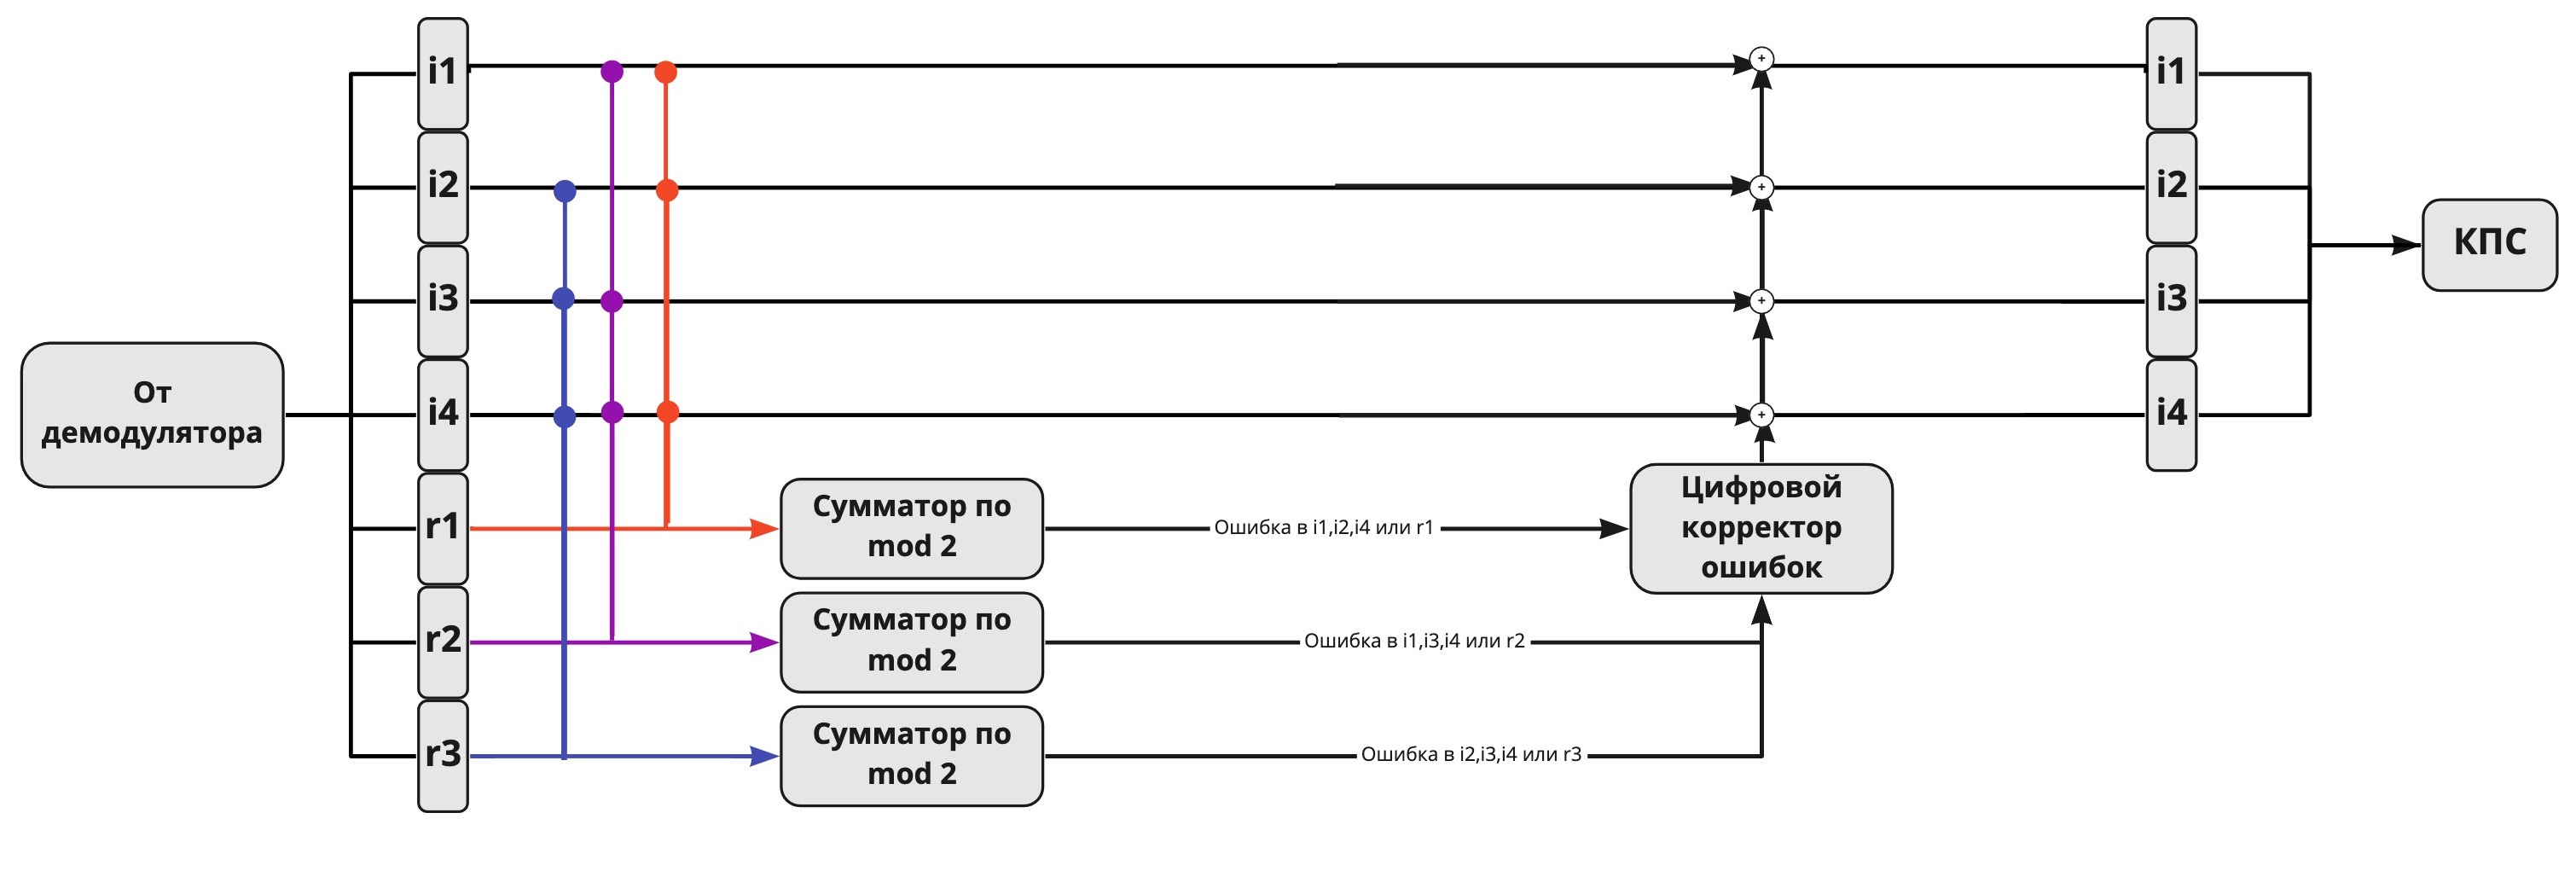
\includegraphics[scale=0.17]{n1.jpg}
\subsection{Задание 2}
Показать, исходя из выбранных вариантов сообщений, имеются ли в принятом сообщении ошибки,
и если имеются, то какие.
\paragraph{№35}
\hfill \break
\FloatBarrier
\begin{table}[h!]
  \begin{tabular}{|c|c|c|c|c|c|c|c|c|}
  \hline
                       & 1                         & 2                         & 3                         & 4                         & 5                         & 6                         & 7                         &      \\ \hline
                       & 0                         & 1                         & 1                         & 1                         & 0                         & 1                         & 0                         &      \\ \hline
  $2^x$ & $r_1$                     & $r_2$                      & $i_1$                      & $r_3$                      & $i_2$                      & $i_3$                      & $i_4$                      & S    \\ \hline
  1                    & \cellcolor[HTML]{32CB00}X &                           & \cellcolor[HTML]{32CB00}X &                           & \cellcolor[HTML]{32CB00}X &                           & \cellcolor[HTML]{32CB00}X & $s_1$ \\ \hline
  2                    &                           & \cellcolor[HTML]{34CDF9}X & \cellcolor[HTML]{34CDF9}X &                           &                           & \cellcolor[HTML]{34CDF9}X & \cellcolor[HTML]{34CDF9}X & $s_2$ \\ \hline
  4                    &                           &                           &                           & \cellcolor[HTML]{FFCC67}X & \cellcolor[HTML]{FFCC67}X & \cellcolor[HTML]{FFCC67}X & \cellcolor[HTML]{FFCC67}X & $s_3$ \\ \hline
  \end{tabular}
\end{table}
\begin{flushleft}
  $s_1 = r_1\oplus i_1 \oplus i_2 \oplus i_4 = 0 \oplus 1 \oplus 0 \oplus 0 = 1 $\\
  $s_2 = r_2\oplus i_1 \oplus i_3 \oplus i_4 = 1 \oplus 1 \oplus 1 \oplus 0 = 1 $\\
  $s_3 = r_3\oplus i_2 \oplus i_3 \oplus i_4 = 1 \oplus 0 \oplus 1 \oplus 0 = 0 $\\
\end{flushleft}
Ошибка в бите $i_1$\\
Правильное сообщение: $0010$
\newpage
\paragraph{№62}
\hfill \break
\FloatBarrier
\begin{table}[h!]
  \begin{tabular}{|c|c|c|c|c|c|c|c|c|}

  \hline
                       & 1                         & 2                         & 3                         & 4                         & 5                         & 6                         & 7                         &      \\ \hline
                       & 0                         & 1                         & 0                         & 1                         & 1                         & 0                         & 0                         &      \\ \hline
  $2^x$ & $r_1$                             & $r_2$                      & $i_1$                      & $r_3$                     & $i_2$                      & $i_3$                      & $i_4$                      & S    \\ \hline
  1                    & \cellcolor[HTML]{32CB00}X &                           & \cellcolor[HTML]{32CB00}X &                           & \cellcolor[HTML]{32CB00}X &                           & \cellcolor[HTML]{32CB00}X & $s_1$ \\ \hline
  2                    &                           & \cellcolor[HTML]{34CDF9}X & \cellcolor[HTML]{34CDF9}X &                           &                           & \cellcolor[HTML]{34CDF9}X & \cellcolor[HTML]{34CDF9}X & $s_2$ \\ \hline
  4                    &                           &                           &                           & \cellcolor[HTML]{FFCC67}X & \cellcolor[HTML]{FFCC67}X & \cellcolor[HTML]{FFCC67}X & \cellcolor[HTML]{FFCC67}X & $s_3$ \\ \hline
  \end{tabular}
\end{table}
$s_1 = r_1\oplus i_1 \oplus i_2 \oplus i_4 = 0 \oplus 0 \oplus 1 \oplus 0 = 1 $\\
$s_2 = r_2\oplus i_1 \oplus i_3 \oplus i_4 = 1 \oplus 0 \oplus 0 \oplus 0 = 1 $\\
$s_3 = r_3\oplus i_2 \oplus i_3 \oplus i_4 = 1 \oplus 1 \oplus 0 \oplus 0 = 0 $\\
Ошибка в бите $i_1$\\
Правильное сообщение: $1100$
\paragraph{№89}
\hfill \break
\FloatBarrier
\begin{table}[h!]
  \begin{tabular}{|c|c|c|c|c|c|c|c|c|}

  \hline
                       & 1                         & 2                         & 3                         & 4                         & 5                         & 6                         & 7                         &      \\ \hline
                       & 0                         & 1                         & 0                         & 1                         & 1                         & 1                         & 0                         &      \\ \hline
  $2^x$ & $r_1$                             & $r_2$                      & $i_1$                      & $r_3$                     & $i_2$                      & $i_3$                      & $i_4$                      & S    \\ \hline
  1                    & \cellcolor[HTML]{32CB00}X &                           & \cellcolor[HTML]{32CB00}X &                           & \cellcolor[HTML]{32CB00}X &                           & \cellcolor[HTML]{32CB00}X & $s_1$ \\ \hline
  2                    &                           & \cellcolor[HTML]{34CDF9}X & \cellcolor[HTML]{34CDF9}X &                           &                           & \cellcolor[HTML]{34CDF9}X & \cellcolor[HTML]{34CDF9}X & $s_2$ \\ \hline
  4                    &                           &                           &                           & \cellcolor[HTML]{FFCC67}X & \cellcolor[HTML]{FFCC67}X & \cellcolor[HTML]{FFCC67}X & \cellcolor[HTML]{FFCC67}X & $s_3$ \\ \hline
  \end{tabular}
\end{table}
$s_1 = r_1\oplus i_1 \oplus i_2 \oplus i_4 = 0 \oplus 0 \oplus 1 \oplus 0 = 1 $\\
$s_2 = r_2\oplus i_1 \oplus i_3 \oplus i_4 = 1 \oplus 0 \oplus 1 \oplus 0 = 0 $\\
$s_3 = r_3\oplus i_2 \oplus i_3 \oplus i_4 = 1 \oplus 1 \oplus 1 \oplus 0 = 1 $\\
Ошибка в бите $i_2$\\
Правильное сообщение: $0010$
\paragraph{№4}
\hfill \break
\FloatBarrier
\begin{table}[h!]
  \begin{tabular}{|c|c|c|c|c|c|c|c|c|}

  \hline
                       & 1                         & 2                         & 3                         & 4                         & 5                         & 6                         & 7                         &      \\ \hline
                       & 0                         & 1                         & 0                         & 0                         & 0                         & 0                         & 0                         &      \\ \hline
  $2^x$ & $r_1$                             & $r_2$                      & $i_1$                      & $r_3$                     & $i_2$                      & $i_3$                      & $i_4$                      & S    \\ \hline
  1                    & \cellcolor[HTML]{32CB00}X &                           & \cellcolor[HTML]{32CB00}X &                           & \cellcolor[HTML]{32CB00}X &                           & \cellcolor[HTML]{32CB00}X & $s_1$ \\ \hline
  2                    &                           & \cellcolor[HTML]{34CDF9}X & \cellcolor[HTML]{34CDF9}X &                           &                           & \cellcolor[HTML]{34CDF9}X & \cellcolor[HTML]{34CDF9}X & $s_2$ \\ \hline
  4                    &                           &                           &                           & \cellcolor[HTML]{FFCC67}X & \cellcolor[HTML]{FFCC67}X & \cellcolor[HTML]{FFCC67}X & \cellcolor[HTML]{FFCC67}X & $s_3$ \\ \hline
  \end{tabular}
\end{table}
$s_1 = r_1\oplus i_1 \oplus i_2 \oplus i_4 = 0 \oplus 0 \oplus 0 \oplus 0 = 0 $\\
$s_2 = r_2\oplus i_1 \oplus i_3 \oplus i_4 = 1 \oplus 0 \oplus 0 \oplus 0 = 1 $\\
$s_3 = r_3\oplus i_2 \oplus i_3 \oplus i_4 = 0 \oplus 0 \oplus 0 \oplus 0 = 0 $\\
Ошибка в бите $r_2$\\
Правильное сообщение: $0000$
\subsection{Задание 3}
Показать, исходя из выбранных вариантов сообщений, имеются ли в принятом сообщении ошибки,
и если имеются, то какие.
\paragraph{№40}
\hfill \break
\FloatBarrier
\begin{table}[!h]
  \begin{tabular}{|c|c|c|c|c|c|c|c|c|c|c|c|c|c|c|c|c|}
  \hline
        & 1                         & 2                         & 3                         & 4                         & 5                         & 6                         & 7                         & 8                         & 9                         & 10                        & 11                        & 12                        & 13                        & 14                        & 15                        &       \\ \hline
        & 0                         & 1                         & 0                         & 1                         & 0                         & 1                         & 0                         & 1                         & 0                         & 0                         & 0                         & 0                         & 0                         & 1                         & 0                         &       \\ \hline
  $2^2$ & $r_1$                     & $r_2$                     & $i_1$                     & $r_3$                     & $i_2$                     & $i_3$                     & $i_4$                     & $r_4$                     & $i_5$                     & $i_6$                     & $i_7$                     & $i_8$                     & $i_9$                     & $i_{10}$                    & $i_{11}$                    & S     \\ \hline
  1     & \cellcolor[HTML]{32CB00}X &                           & \cellcolor[HTML]{32CB00}X &                           & \cellcolor[HTML]{32CB00}X &                           & \cellcolor[HTML]{32CB00}X &                           & \cellcolor[HTML]{32CB00}X &                           & \cellcolor[HTML]{32CB00}X &                           & \cellcolor[HTML]{32CB00}X &                           & \cellcolor[HTML]{32CB00}X & $s_1$ \\ \hline
  2     &                           & \cellcolor[HTML]{34CDF9}X & \cellcolor[HTML]{34CDF9}X &                           &                           & \cellcolor[HTML]{34CDF9}X & \cellcolor[HTML]{34CDF9}X &                           &                           & \cellcolor[HTML]{34CDF9}X & \cellcolor[HTML]{34CDF9}X &                           &                           & \cellcolor[HTML]{34CDF9}X & \cellcolor[HTML]{34CDF9}X & $s_2$ \\ \hline
  4     &                           &                           &                           & \cellcolor[HTML]{FFCC67}X & \cellcolor[HTML]{FFCC67}X & \cellcolor[HTML]{FFCC67}X & \cellcolor[HTML]{FFCC67}X &                           &                           &                           &                           & \cellcolor[HTML]{FFCC67}X & \cellcolor[HTML]{FFCC67}X & \cellcolor[HTML]{FFCC67}X & \cellcolor[HTML]{FFCC67}X & $s_3$ \\ \hline
  8     &                           &                           &                           &                           &                           &                           &                           & \cellcolor[HTML]{FD6864}X & \cellcolor[HTML]{FD6864}X & \cellcolor[HTML]{FD6864}X & \cellcolor[HTML]{FD6864}X & \cellcolor[HTML]{FD6864}X & \cellcolor[HTML]{FD6864}X & \cellcolor[HTML]{FD6864}X & \cellcolor[HTML]{FD6864}X & $s_4$ \\ \hline
  \end{tabular}
\end{table}
$s_1 = r_1\oplus i_1 \oplus i_2 \oplus i_4 \oplus i_5 \oplus i_7 \oplus i_9 \oplus i_{11} = 0 \oplus 0 \oplus 0 \oplus 0 \oplus 0 \oplus 0 \oplus 0 \oplus 0= 0 $\\
$s_2 = r_2\oplus i_1 \oplus i_3 \oplus i_4 \oplus i_6 \oplus i_7 \oplus i_{10} \oplus i_{11} = 1 \oplus 0 \oplus 1 \oplus 0 \oplus 0 \oplus 0 \oplus 1 \oplus 0 = 1 $\\
$s_3 = r_3\oplus i_2 \oplus i_3 \oplus i_4 \oplus i_8\oplus i_9 \oplus i_{10} \oplus i_{11}= 1 \oplus 0 \oplus 1 \oplus 0 \oplus 0 \oplus 0 \oplus 1 \oplus 0  = 1 $\\
$s_4 = r_4\oplus i_5 \oplus i_6 \oplus i_7 \oplus i_8\oplus i_9 \oplus i_{10} \oplus i_{11}= 1 \oplus 0 \oplus 0 \oplus 0 \oplus 0 \oplus 0 \oplus 1 \oplus 0  = 0 $\\
Ошибка в бите $i_3$\\
Правильное сообщение: $00000000010$
\subsection{Задание 4}
Сложить номера всех 5 вариантов заданий. Умножить полученное число на 4. Принять данное число как число информационных разрядов
в передаваемом сообщении. Вычислить для данного числа минимальное число проверочных разрядов и коэффициент избыточности.\\
\hfill \break
\textbf{Число информационных разрядов:} $4\cdot(35+62+89+4+40)=920$\\
\textbf{Минимальное число проверочных разрядов:}\\
$2^r \geq r + i + 1$\\
$2^9 = 512 < 9 + 920 + 1 < 10 + 920 + 1 < 2^{10}$\\
$\Rightarrow $ Минимальное число проверочных разрядов = 10\\
\textbf{Коэффициент избыточности:}\\
\hfill \break
$k = \frac{\text{число проверочных разрядов}}{\text{общее число разрядов}}$\\
$k = \frac{10}{930}=\frac{1}{93} \approx 0,01 $
\newpage
\subsection{Задание 5}
Написать программу на любом языке программирования, которая на вход из командной строки получает набор из 7 цифр "0" и "1" записанных подряд, анализирует это сообщение на основе классического кода Хэминга (7,4), а затем выдаёт
правильное сообщение(только информационные биты) и указывает бит с ошибкой при его наличии.
\paragraph{Код}
\hfill \break
\lstloadlanguages{Python}
\definecolor{mygray}{RGB}{120,120,120}
\lstset{extendedchars =/true,
breaklines=true,
basicstyle=\ttfamily\fontsize{9pt}{9pt}\selectfont,
commentstyle=\color{mygray},
keywordstyle=\color{blue},
keepspaces=true,
showstringspaces=false}
\lstinputlisting[language=Python,numbers=left]{prog.py}
\paragraph{Результат выполнения:}
\hfill \break
\begin{lstlisting}[basicstyle=\ttfamily\fontsize{12pt}{12pt}\selectfont]
  0101100
  Ошибка в бите i1
  Правильное сообщение:1100  
\end{lstlisting}
\section{Вывод:}
В этой лабораторной работе я познакомился помехоустойчивыми кодами. Научился работать с кодом Хэминга.
\end{flushleft}
\begin{thebibliography}{2}
\addcontentsline{toc}{section}{\bibname}
\bibitem {1}
\href{https://www.youtube.com/watch?v=X8jsijhllIA}{«How to send a self-correcting message (Hamming codes)»} --- 3Blue1Brown
\bibitem {2}
\href{https://www.youtube.com/watch?v=h0jloehRKas&t=0s}{What is error correction? Hamming codes in hardware} --- Ben Eater
\end{thebibliography}
\end{document}